\chapter{Requirements and System Architecture}
\label{chap:architecture}

\section{Functional requirements}

\begin{longtable}{p{0.14\textwidth}p{0.78\textwidth}}
\caption{Functional requirements specification}
\label{tab:functional-requirements}\\
\toprule
\textbf{ID} & \textbf{Requirement Description}\\
\midrule
\endfirsthead
\toprule
\textbf{ID} & \textbf{Requirement Description}\\
\midrule
\endhead
FR-01 & Validate and process required IEEE-CIS transaction and identity CSV files.\\
FR-02 & Produce train, validation, holdout, and unlabeled model-ready datasets.\\
FR-03 & Preserve canonical feature order and preprocessing metadata.\\
FR-04 & Compare binary classifiers using validation PR-AUC metrics.\\
FR-05 & Score transactions and return probability, risk score, version, and explanations.\\
FR-06 & Persist scored transactions and human review outcomes.\\
FR-07 & Filter, sort, paginate, and inspect transaction records.\\
FR-08 & Import CSV and load processed datasets with progress reporting.\\
FR-09 & Support review approval/rejection and fraud/legitimate labels.\\
FR-10 & Present risk, SHAP evidence, and model state in a browser interface.\\
\bottomrule
\end{longtable}

The functional requirements define what a user can do with the system. They
begin with validated data and model-ready outputs, then continue through
scoring, persistence, filtering, import, and analyst review. This ordering
reflects the dependency chain in the implementation: the review interface
cannot provide a reliable decision unless the scoring contract and persisted
transaction record exist first.

\section{Quality requirements}

\begin{longtable}{p{0.14\textwidth}p{0.78\textwidth}}
\caption{Quality requirements specification}
\label{tab:quality-requirements}\\
\toprule
\textbf{ID} & \textbf{Requirement Description}\\
\midrule
\endfirsthead
\toprule
\textbf{ID} & \textbf{Requirement Description}\\
\midrule
\endhead
QR-01 & Temporal leakage control and non-overlapping chronological splits.\\
QR-02 & Reproducible schema and feature contracts.\\
QR-03 & Version-aware model artifacts and rollback capability.\\
QR-04 & Explainable tree-model predictions via TreeSHAP.\\
QR-05 & Local containerized deployment with bounded data mounts.\\
QR-06 & Automated subsystem test suite.\\
QR-07 & Auditable experiment and promotion lineage.\\
QR-08 & Durable background job operations.\\
QR-09 & Role-based authentication, authorization, and audit logging.\\
QR-10 & Real-time production latency and drift monitoring.\\
\bottomrule
\end{longtable}

The quality requirements define how the system should behave beyond the basic
feature list. Temporal leakage control and contract verification protect the
validity of the model result, while versioning, explainability, tests, and
lineage protect reproducibility and reviewability. Durable jobs, access control,
audit logging, latency monitoring, and drift monitoring are included as target
requirements even where the current demonstration has not implemented them
fully.

\section{Integrated architecture}

The system integrates batch data preparation, offline ML training, and online inference into an in-process modular monolith. Figure~\ref{fig:final-overall-system} presents the overall architecture and data flow contracts.

The architecture has four cooperating layers. The data-processing layer owns
raw-file discovery, Spark transformations, feature engineering, and model-ready
Parquet output. The model layer consumes that contract, trains and compares
candidates, calibrates the selected challenger, and writes a versioned package.
The backend layer loads the package, validates scoring requests, persists
results, and exposes typed endpoints. The frontend layer presents the risk
decision, explanation, transaction history, and review action to a human user.
The layers are logically decoupled through files and typed interfaces even
though the current deployment packages several of them in one repository and
local Compose environment.

\begin{figure}[H]
\centering
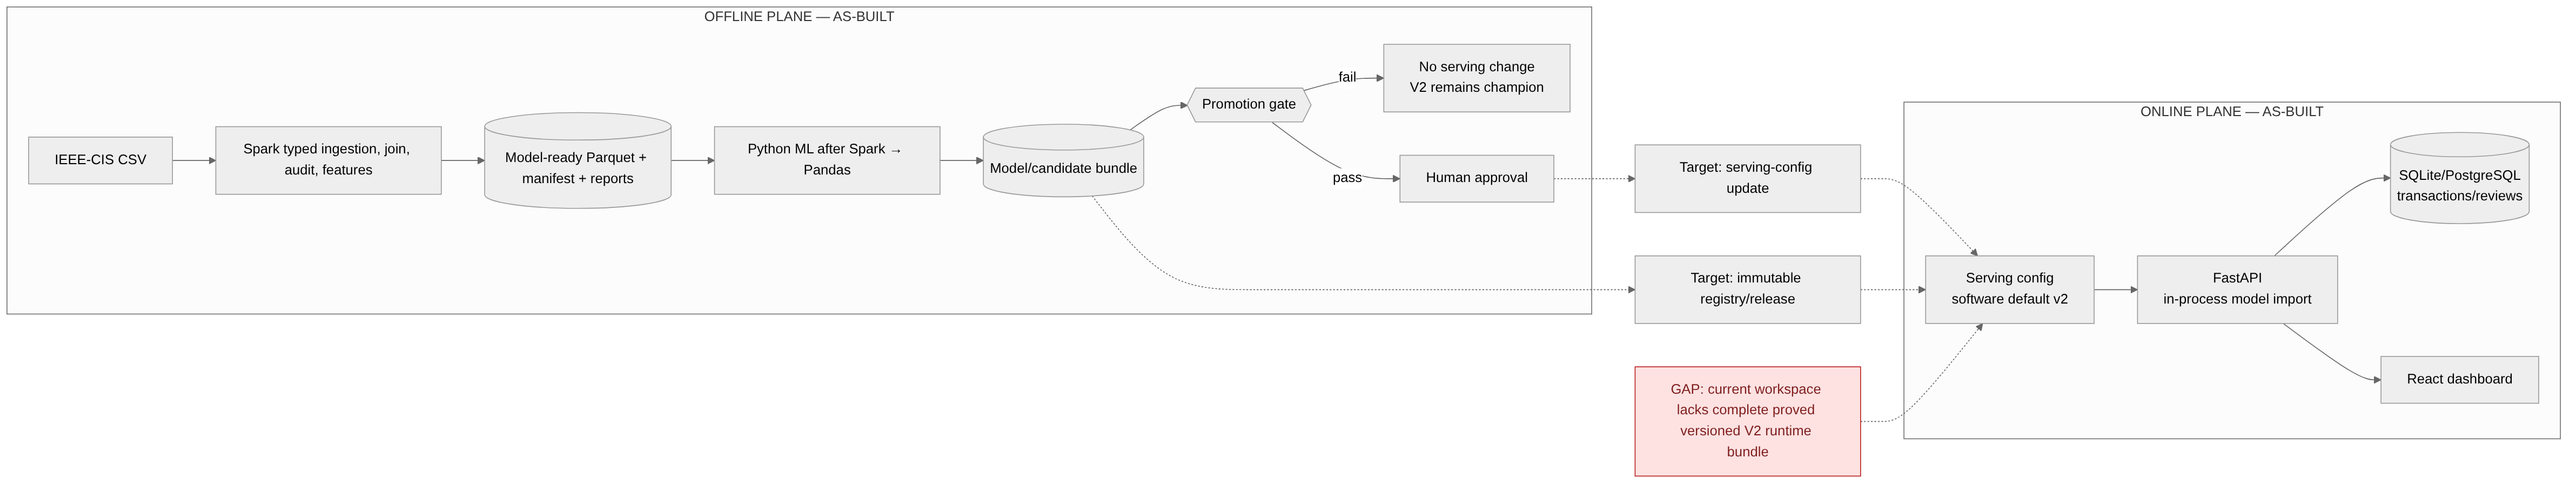
\includegraphics[width=0.85\textwidth,height=0.22\textheight,keepaspectratio]{../../docs/diagrams/final/overall-system-architecture.png}
\caption[Overall system architecture]{Overall system architecture.}
\label{fig:final-overall-system}
\end{figure}


\section{System contracts}

The system enforces three related contracts across its boundaries. The Data Contract defines the canonical 68-feature vector, its ordering, preprocessing metadata, and schema hash; this is the control that prevents the trainer and scorer from silently interpreting the same position as different variables. The Scoring Contract defines the per-transaction request and response, including the fraud probability, the derived risk score, and the TreeSHAP attribution payload. The API Contract then exposes those objects through typed Pydantic models on the backend and corresponding TypeScript types in the frontend. Together, these contracts make the handover between data preparation, model execution, and user interface explicit and testable.

\begin{figure}[H]
\centering
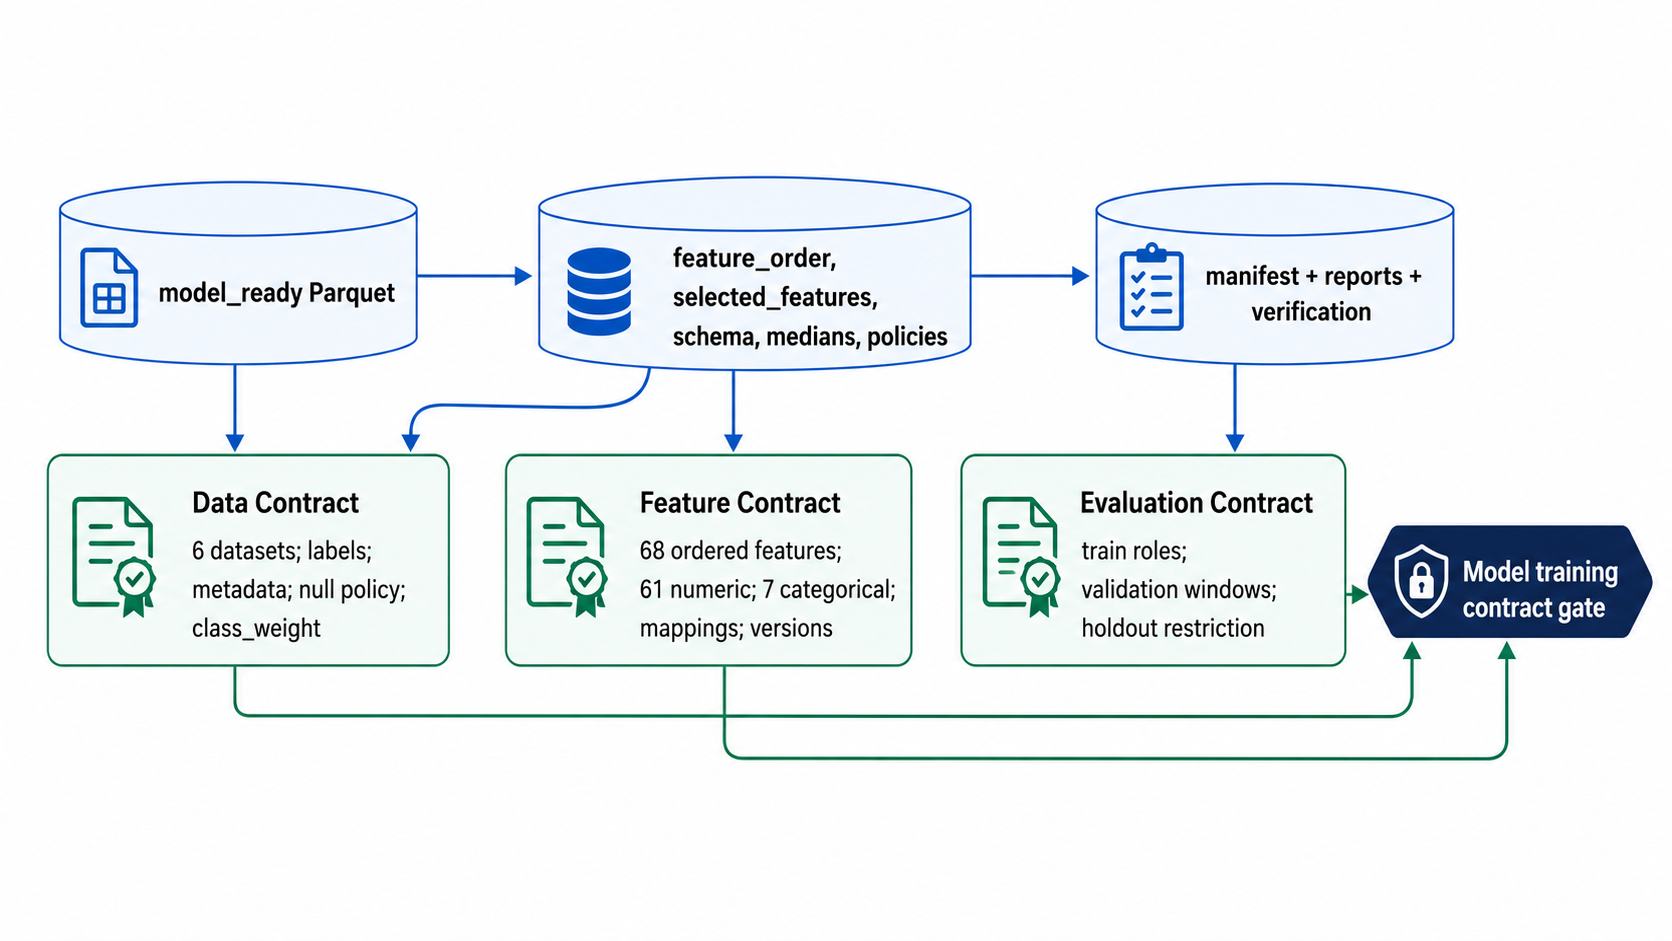
\includegraphics[width=\textwidth,height=0.36\textheight,keepaspectratio]{../../docs/diagrams/final/data-feature-evaluation-contracts.png}
\caption[Data, feature, and evaluation contracts]{Data, feature, and evaluation contracts. Split configuration and training protocol define the Evaluation Contract.}
\label{fig:final-contracts}
\end{figure}


\section{Technology stack used by the group}

Apache Spark and PySpark form the data-processing foundation of the project.
The group uses Spark DataFrames and Spark SQL-style transformations to read
the wide CSV files with explicit schemas, validate identifiers, join
transaction and identity records, calculate distributed summaries, construct
temporal features, and export model-ready data. Spark MLlib is also used for
the DecisionTree baseline, which gives the project a native distributed
machine-learning reference in addition to the Python estimator experiments
\parencite{zaharia2016spark,meng2016mllib,sparkmllibguide}.

Parquet is used as the handover format between data preparation and model
training. Its column-oriented representation preserves schema information and
allows downstream jobs to read only the columns they need, which is more
appropriate for repeated analytical access than passing the original CSV files
between every stage \parencite{sparkparquet}. The repository's data contract
adds the project-specific guarantees that Parquet alone cannot provide,
including the canonical 68-feature order, imputation values, categorical
mappings, and schema hash.

The modelling layer compares Logistic Regression, LightGBM, XGBoost, and
CatBoost. Logistic Regression provides a linear reference, while the boosting
families model nonlinear interactions in a wide tabular feature space. CatBoost
is particularly relevant because its documentation describes native handling
of categorical features and feature combinations, although this project still
passes a frozen contract to the estimator and records the exact preprocessing
state used in its candidate package \parencite{prokhorenkova2018catboost,catboostdocs}.
The group uses isotonic calibration for the selected candidate so that the
returned probability is evaluated separately from the ranking score. It uses
SHAP/TreeSHAP at request time to expose local feature contributions; SHAP values
are treated as additive explanations of the model output, not as causal proof
\parencite{lundberg2017shap}.

FastAPI provides the backend HTTP service and Pydantic validation layer. The
service loads the packaged model without starting Spark for every request,
returns probability, risk score, policy band, decision, model version, and
explanation fields, and persists scoring and review records through the
database layer. PostgreSQL is the durable database target for the full stack,
while SQLite is retained as a lightweight local configuration for development
and demonstration.

React and TypeScript provide the browser dashboard. The group uses typed API
responses to render a transaction queue, risk badges, score details, SHAP
charts, import progress, and analyst review actions. This frontend is not a
separate analytical model; it is the human-facing layer that turns the backend
contract into a review workflow. Docker Compose packages the local services,
including preprocessing, backend, database, and frontend profiles, so that the
team can demonstrate the complete path in a controlled environment
\parencite{fastapi,postgresql,react,dockerdocs}.

MLflow is used for experiment and model-lineage information in the training
workflow. The recorded metadata helps distinguish a historical serving
artifact from a current challenger, preserve calibration and threshold
evidence, and evaluate promotion gates. The group deliberately keeps the
promotion decision separate from the model-training library: an experiment can
complete successfully while still failing the holdout-quality gate and
remaining unpromoted \parencite{mlflow}.

\section{Implementation parameters and reproducibility}

Table~\ref{tab:implementation-parameters} records the concrete implementation
parameters used by the project. Version ranges are reported from the repository
manifests, while values such as Spark memory, shuffle partitions, ratios, and
random seed are taken from the pipeline configuration.

\begin{table}[H]
\centering
\small
\rowcolors{2}{ReportGray!25}{white}
\caption{Implementation parameters and reproducibility settings}
\label{tab:implementation-parameters}
\begin{tabularx}{\textwidth}{p{0.30\textwidth}X}
\toprule
\textbf{Parameter} & \textbf{Recorded value and interpretation}\\
\midrule
Python runtime & Model and backend packages require Python \val{3.11} or newer; no single patch version is claimed.\\
Spark runtime & The model package and Docker training image use Apache Spark/PySpark \val{3.5.1}.\\
Data preparation & Spark \texttt{local[4]}, driver memory \val{8~GB}, driver result limit \val{1~GB}, shuffle partitions \val{64}, default parallelism \val{8}.\\
Cluster configuration & Standalone Spark master on port \val{7077}; two workers, each configured with \val{2} cores and \val{4~GB} memory.\\
Split policy & Chronological ratios of \val{70\%}/\val{15\%}/\val{15\%} for train, validation, and holdout.\\
Randomness & Imbalance sampling seed \val{42}; model-family estimators use the same seed where supported.\\
Missingness policy & Missingness bands use thresholds \val{0.20}, \val{0.70}, and \val{0.95}; quantile summaries use relative error \val{0.01}.\\
Serving stack & FastAPI/Uvicorn on port \val{8000}; React/Vite on \val{5173}; PostgreSQL \val{16} on \val{5432}; optional Adminer on \val{8081}.\\
Feature handover & Frozen canonical vector of \val{68} features with preprocessing metadata, categorical mappings, feature order, and schema hash.\\
\bottomrule
\end{tabularx}
\end{table}

The repository contains two dependency manifests with different PySpark
constraints: the model package and preprocessing environment pin PySpark to
\val{3.5.1}, whereas the generic root \texttt{requirements.txt} declares
\texttt{pyspark>=4.2.0}. The controlled training and Docker path used for the
reported results is the former \val{3.5.1} environment. This discrepancy is
retained as a reproducibility limitation and should be resolved before a clean
installation is published as the single official environment.

The model manifest declares CatBoost \val{1.2.10} or newer, LightGBM
\val{4.7.0} or newer, XGBoost \val{3.2.0} or newer, scikit-learn
\val{1.9.0} or newer, SHAP \val{0.51.0} or newer, and MLflow \val{3.3.0} or
newer. The backend manifest declares FastAPI \val{0.139.2} or newer,
Uvicorn \val{0.51.0} or newer, SQLAlchemy \val{2.0.36} or newer, and psycopg
\val{3.2.3} or newer. These are dependency constraints rather than a claim
that every component was independently benchmarked at its latest release.

\section{Architectural tradeoffs}

\begin{table}[H]
\centering
\small
\setlength{\tabcolsep}{0pt}
\rowcolors{2}{ReportGray!25}{white}
\caption{Major architectural tradeoffs}
\label{tab:architecture-tradeoffs}
\begin{tabularx}{\textwidth}{p{0.25\textwidth}XX}
\toprule
\textbf{Choice} & \textbf{Benefit} & \textbf{Cost}\\
\midrule
Monorepo and path dependency & Simple handoff and one Compose stack & Backend inherits model dependencies\\
Spark then pandas & Scalable preparation and familiar estimators & Driver-memory training ceiling\\
Fixed backend risk bands & Stable UI and simple tests & Not tied to model operating evidence\\
In-memory jobs & Minimal infrastructure & Lost on restart and single-worker only\\
SQLite local default & Fast developer startup & Different operational behavior from PostgreSQL\\
Heuristic fallback & Demo continuity & Can conceal model loading failures\\
Manual TypeScript types & No generator setup & Contract drift risk\\
\bottomrule
\end{tabularx}
\setlength{\tabcolsep}{4pt}
\end{table}

The trade-off table shows that the current architecture favours clarity and
local reproducibility over independent scaling. Spark provides a suitable
processing boundary, but moving to a single-node Python estimator creates a
memory ceiling. In-memory jobs and a heuristic fallback keep the demonstration
available with minimal infrastructure, but they can lose work or conceal
failures after a restart. These are deliberate compromises for the academic
scope and are not presented as final production decisions.

These trade-offs reflect the project's academic and demonstration objectives.
Using Spark for preparation provides an appropriate distributed processing
boundary and makes joins, windows, and aggregations explicit. Keeping the
estimator stage in Python simplifies experimentation with several model
families and calibration libraries, but it also means that the full training
matrix must fit within the driver and model-training environment. Likewise,
the modular monolith reduces integration overhead and makes a complete demo
easy to run locally, but it does not provide the isolation, independent
scaling, or failure containment expected from a production platform. The
architecture is therefore intentionally useful for audit and demonstration,
not presented as the final deployment topology.

\section{Main source code components}

Table~\ref{tab:main-source-files} outlines the primary source implementation files and core responsibilities across project components.

\begin{table}[H]
\centering
\small
\rowcolors{2}{ReportGray!25}{white}
\caption{Main Source Files and Component Responsibilities}
\label{tab:main-source-files}
\begin{tabularx}{\textwidth}{p{0.24\textwidth}p{0.34\textwidth}X}
\toprule
\textbf{Component} & \textbf{Module reference} & \textbf{Responsibility}\\
\midrule
Spark Preprocessing & Preprocessing Pipeline & Schema ingestion, left join, leakage-free transformation, Parquet export\\
Data Verifier & Verification Engine & Validates dataset row counts, schema hash, split overlap, verification report\\
Model Training & Estimator Training Module & Single-node candidate training, tuning, calibration, holdout evaluation\\
Backend Scoring & FastAPI Scoring Service & Artifact loading, probability scoring, SHAP calculation, FastAPI endpoints\\
Frontend Dashboard & React UI Dashboard & React UI, risk queue, SHAP feature rendering, analyst review workflow\\
Docker Deployment & Multi-container Orchestration & Multi-container service orchestration (backend, frontend, db, preprocessing)\\
\bottomrule
\end{tabularx}
\end{table}

The source-component table maps repository responsibilities to the major
subsystems. It shows that validation is implemented as its own evidence layer,
rather than being hidden inside model training, and that the backend and
frontend consume explicit scoring and API contracts. This separation makes a
feature-pipeline change easier to check before it reaches the user interface.

\section{Distributed Spark execution evidence}

Table~\ref{tab:spark-execution-evidence} presents the Spark execution configurations together with the validation evidence and reported outcomes. This expands the original infrastructure-only view so that the table records not only how the pipeline was configured, but also what was checked and what the run produced.

\begin{table}[H]
\centering
\small
\rowcolors{2}{ReportGray!25}{white}
\caption{Distributed Spark Execution and Validation Evidence}
\label{tab:spark-execution-evidence}
\setlength{\tabcolsep}{0pt}
\begin{tabularx}{\textwidth}{>{\raggedright\arraybackslash}p{0.17\textwidth} >{\raggedright\arraybackslash}p{0.17\textwidth} >{\raggedright\arraybackslash}p{0.16\textwidth} X}
\toprule
\textbf{Stage} & \textbf{Configuration} & \textbf{Output} & \textbf{Validation and reported result}\\
\midrule
Local Spark preprocessing & local mode, one worker, four CPUs, 8GB memory & Model-ready Parquet and reports & \val{94} checks passed and zero failed; source, schema, join, split, and feature-contract checks are ready for downstream training.\\
Configured cluster mode & Spark master on port 7077, two workers, four CPUs, 8GB memory & Cluster deployment specification & Configuration is implemented; a clean end-to-end distributed runtime was not independently verified.\\
Chronological validation & TransactionDT ordering from train to validation to holdout & Three labelled windows & Train: \val{412,956}; validation: \val{88,486}; holdout: \val{89,098}. Fraud rates are \val{3.5166\%}, \val{3.4310\%}, and \val{3.4849\%}.\\
Model-ready handover & Canonical \val{68}-feature vector and schema hash & Training contract & Handover is marked ready; no identifier or split-overlap failure was recorded.\\
\bottomrule
\end{tabularx}
\setlength{\tabcolsep}{4pt}
\end{table}

\textit{Note: Cluster configuration is implemented, but a clean end-to-end distributed runtime was not independently verified.}
